\documentclass[a4paper,12pt]{book}
%\usepackage[utf8]{inputenc}
\usepackage{graphicx}

\usepackage{tikz}
\usetikzlibrary{arrows}


\usepackage{xepersian}


\settextfont{Nazli}

\setlatintextfont[Scale=0.8]{Times New Roman}

\begin{document}

\author{دکتر علی عباسی مولایی\\
	دانشیار دانشگاه دامغان، دانشکده ریاضی و علوم کامپیوتر  \\ 
	\and
	 گرداوری توسط \\
	  مهندس متین نصرتی، دانشگاه دامغان
  }
\title{جزوه درس بهینه سازی شبکه پیشرفته}
\date{نیمسال تحصیلی دوم 1401-1402}
\maketitle
\frontmatter

\tableofcontents

\mainmatter
\chapter[مقدمات]{مقدمات و مفاهیم اولیه شبکه}

\section[مفهوم هر مسئله]{مفهوم هر مسئله\\}{
	
	
	~~پیش از شروع بهتر است کمی با مسئله هایی که در فهرست آمده آشنا شده و مفهوم آنها را درک کنیم:
	به نصویر \ref{dummy_1} توجه کنید:\\
\begin{figure}[h!]
	\centering
		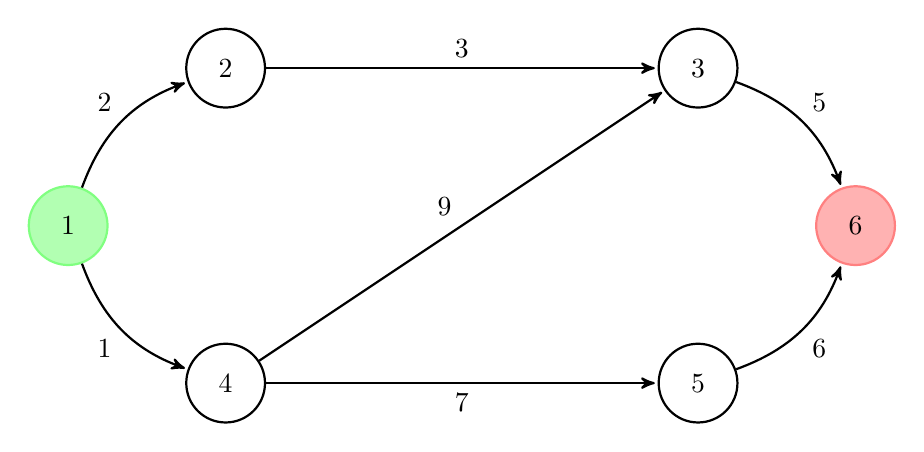
\begin{tikzpicture}[->,>=stealth',shorten >=1pt,auto,thick] 
			
			\node (1)	at	(-5,3) [circle,draw=green!50,fill=green!30,thick,inner sep=0pt,minimum size=1cm] {1};
			\node (3)	at 	(3,5) [circle,draw=black,inner sep=0pt,minimum size=1cm]{3};
			\node (2)	at 	(-3,5) [circle,draw=black,inner sep=0pt,minimum size=1cm]{2};
			\node (5)	at 	(3,1) [circle,draw=black,inner sep=0pt,minimum size=1cm]{5};
			\node (4)	at	(-3,1) [circle,draw=black,inner sep=0pt,minimum size=1cm]{4};
			\node (6)	at 	(5,3) [circle,draw=red!	50,fill=red!30,thick,inner sep=0pt,minimum size=1cm]{6};

			\draw (1)[bend left=25] to node []{2} (2);
			\draw (1) [bend right=25] to node [swap]{1} (4);
			\draw (2) to node {3} (3);
			\draw (3)[bend left=25]  to node {5} (6);
			\draw (4) to node {9} (3);
			\draw (4) to node [swap] {7} (5);
			\draw (5)[bend right=25]  to node[swap] {6} (6);		
			
			

		\end{tikzpicture}
		\label{dummy_1}
		\centering\caption[شبکه نمونه]{یک شبکه دارای ظرفیت:گره  \footnotemark[1] سبز رنگ بیانگر مبدا و گره قرمز بیانگر مقصد است. به مبدا و قصد هر یال\footnotemark[2]  توجه کنید .}
	\end{figure}\
	\footnotetext[1]{Node نود  نیز گفته میشود.}
	\footnotetext[2]{Arrow مسیر یا پیکان نیز گفته میشود.}	

	\begin{description}
		\item[\textbf{مسئله کوتاه ترین مسیر:}‍] در این نوع مسائل هدف ما پیدا کردن کوتاه ترین مسیر بین دو گره فارِغ از هزینه آن است.
		\item[\textbf{مسئله ماکسیموم جریان:}] مسئله همواره در یک شبکه دارای ظرفیت مطرح میشود.هدف این است بیشترین جریان ممکن  از گره مبدا به گره مقصد ممکن است را بیابیم.
		\item [\textbf{مسئله مینیموم هزینه جریان:}] این مسئله به نوعی ترکیب دو مسئله ی بالایی می‌باشد. مسئله همواره در یک محیط ظرفیت دار می‌باشد.هدف دراین مسائل این است که کوتاه ترین مسیر ممکن از مبدا به مقصد را در حالی بیابیم کهکم هزینه ترین مسیر هم باشد.
	\end{description}
 \section*{روند حل مسئله\\}
 شکل \ref{dummy_1} برای حل مسئله ی کوتاهترین مسیر در نظر بگیرید:\\ مسئله را را بری حل کوتاه ترین مسیر اجرا میکنید.\\روند حل به صورت مستقیم\footnotemark به شکل زیر است
 \footnotetext{روش حل مستقیم یا روش حل قدرتمند یا brutal :روند حلی که تمام حالات ممکن در آن بررسی میشود.}
 \begin{enumerate}
 	\item مسیریابی از گره یک تا 6 را انجام ده
 	\item طول هر مسیر را محاسبه کن
 	\item کوتاه‌ترین مسیر را انتخاب کن.
 \end{enumerate}
روش حل به صورت مستبقم زیاد مقبول و مناسب نیست؛زیرا ممکن است تمام حالات ممکن زیاد باشد و همین امر باعث هزینه زمانی زیادی شود. هر چند این روش حتما جواب دارد و در صورت وجود جواب بهترین جواب را ارائه می‌کند اما {\underline{زمان رسیدن به جواب}} میتواند بسیار زیاد باشد.
بدین سبب  قصد داریم در این درس الگوریتم هایی را بررسی کنیم که زمان محاسبه آن کم یا قابل قبول باشد.

\section[مفاهیم شبکه]{مفاهیم اولیه شبکه \\}
به تعاریف بنیادی این  درس می‌پردازیم:
\begin{description}
	\item[شبکه\footnotemark :]  یک گراف\footnotemark می‌باشد که همواره ۳ مشخصه دارد و به بدین شکل نمایش داده می‌شود:  \begin{flushleft}
\textbf{		{G(N,A)}}
	\end{flushleft}
که در آن G معرف نام شبکه، N معرف گره های شبکه و A معرف زوج مرتب هایی می‌باشد که یال‌های شبکه نمایش میدهند.

\begin{figure}[t]
	\centering
	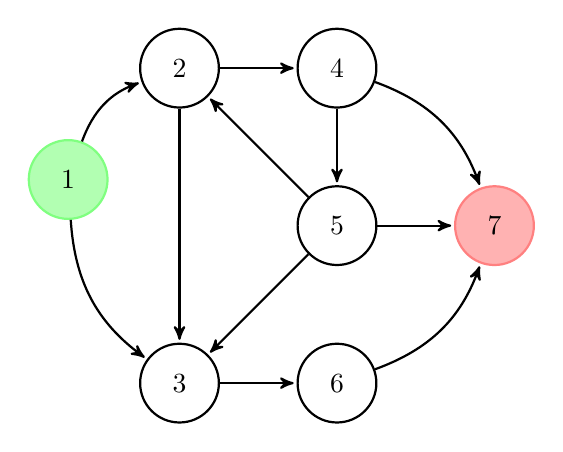
\begin{tikzpicture}[->,>=stealth',node distance=2cm,shorten >=1pt,auto,thick,mabda/.style={circle,draw=green!50,fill=green!30,thick,inner sep=0pt,minimum size=1cm},maqsad/.style={circle,draw=red!50,fill=red!30,thick,inner sep=0pt,minimum size=1cm},masir/.style={circle,draw=black,inner sep=0pt,minimum size=1cm}]
		\node	[mabda]	(1) {1};
		\node[masir] (2) [above right of= 1] {2};

		\node[masir] (4) [right of =2]{4};
		\node[masir] (5) [below of =4]{5};
		\node[masir] (6) [below of =5]{6};
		\node[maqsad] (7) [	right of = 5]{7};
		\node[masir] (3) [	left of=6]{3};
		
		\draw (1)[bend left=25]  to node {}(2);
		\draw (1) [bend right=25] to node {}(3);
		\draw (2) to node {}(4);
		\draw (2) to node {}(3);
		\draw (3) to node {}(6);
		\draw (4) to node {}(5);
		\draw (4) [bend left=25]  to node {}(7);
		\draw (5) to node {}(2);
		\draw (5) to node {}(3);
		\draw (5) to node {}(7);
		\draw (6)[bend right=25]  to node {}(7);

		\end{tikzpicture}
\caption{گراف G یک گراف بدون ظرفیت}\label{dummy_2}\end{figure}
به گراف  \ref{dummy_2} توجه کنید:
این گراف به صورت G(N,A) نمایش داده میشود که N={1,2,3,4,5,6,7} وA={(1,2),(1,3),(2,3),(2,4),(3,6),(4,5),(4,5),(5,2),(5,3),(5,7),(6,7)} می‌باشند.
\textbf{تذکر:}در برخی گراف ها مانند گراف \ref{dummy_1}اعدادی بر روی یال ها و گره ها گذاشته می‌شوند که با توجه به فرض مسئله می‌تواند بیانگر ظرفیت، هزینه مسیر، منابع و... باشد.
\end{description}


}
 \chapter[کوتاه ترین مسیر]{مسئله کوتاه ترین مسیر در شبکه}
 	\section[\LR{Label setting algorithm}]{Label setting algorithm}
 	\section[\LR{Label correcting algorithm}]{\LR{Label correcting algorithm}}
 \chapter[ماکسیموم جریان در شبکه]{ماکسیموم جریان در شبکه}
	\section[جریان ها و برش ها]{جریان ها و برش ها}
	\section[\LR{Genetic algorithm path}]{Genetic algorithm path}
	\section[\LR{Labeling algorithm}]{\LR{Labeling algorithm}}
 \chapter[مسئله مینیموم هزینه جریان]{مسئله مینیموم هزینه جریان}
	\section[تعریف مسئله]{تعریف مسئله}
	\section[ارائه الگوریتم برای حل مسئله]{ارائه الگوریتم برای حل مسئله}
\backmatter
% bibliography, glossary and index would go here.

\end{document}